\documentclass[12pt]{iopart}
\pdfoutput=1
\usepackage{iopams}
\usepackage{amssymb, epsfig}
%\usepackage{amsmath, amssymb,epsfig}
\usepackage{latexsym}

%\usepackage[hypertex,hyperindex]{hyperref}
%\usepackage{showkeys}
\usepackage{graphicx}
\usepackage{color}

\newcommand{\pf}{\mbox{pf}}
\newcommand{\vep}{\varepsilon}

\begin{document}

\bibliographystyle{plain}
\def\debproof{\noindent {\bf Proof.} }
\def\finproof{\hfill {\small $\Box$} \\}
%\renewcommand{\theequation}{\arabic{section}.\arabic{equation}}
%\tableofcontents
\makeatletter % `@' now normal "letter"
\@addtoreset{equation}{section}
\makeatother  % `@' is restored as "non-letter"
\renewcommand\theequation{{\thesection}.{\arabic{equation}}}

\title[]{Numerical Tests of RTM for Locally Perturbed Two-layers Media}
\author{ }
\address{}



\maketitle

\newcommand{\eps}{\varepsilon}
\newcommand{\RR}{\mathcal{R}}
\newtheorem{lem}{Lemma}[section]
\newtheorem{prop}{Proposition}[section]
\newtheorem{cor}{Corollary}[section]
\newtheorem{thm}{Theorem}[section]
\newtheorem{rem}{Remark}[section]
\newtheorem{alg}{Algorithm}[section]
\newtheorem{assum}{Assumption}[section]
\newtheorem{definition}{Definition}[section]


\newcounter{RomanNumber}
\newcommand{\MyRoman}[1]{\rm\setcounter{RomanNumber}{#1}\Roman{RomanNumber}}

\newcommand{\bL}{\mathbf{L}}
\newcommand{\bH}{\mathbf{H}}
\newcommand{\bW}{\mathbf{W}}
\newcommand{\bP}{\mathbf{P}}
\newcommand{\bQ}{\mathbf{Q}}
\newcommand{\bp}{\mathbf{p}}
\newcommand{\bq}{\mathbf{q}}
\newcommand{\uL}{u_{_{\rm L}}}
\newcommand{\vL}{v_{_{\rm L}}}
\newcommand{\tuL}{\tilde u_{_{\rm L}}}
\newcommand{\tvL}{\tilde v_{_{\rm L}}}
\newcommand{\fL}{f_{_{\rm L}}}
\newcommand{\gL}{g_{_{\rm L}}}
\newcommand{\bpL}{\bp_{_{\rm L}}}
\newcommand{\bqL}{\bq_{_{\rm L}}}
\newcommand{\tbpL}{\tilde{\bp}_{_{\rm L}}}
\newcommand{\tbqL}{\tilde{\bq}_{_{\rm L}}}
\newcommand{\tbpLf}{\tilde{\bp}_{_{\rm L,1}}}
\newcommand{\tbpLs}{\tilde{\bp}_{_{\rm L,2}}}
\newcommand{\tbqLf}{\tilde{\bq}_{_{\rm L,1}}}
\newcommand{\tbqLs}{\tilde{\bq}_{_{\rm L,2}}}
\newcommand{\bn}{\nu}
\newcommand{\bv}{\mathbf{v}}
\newcommand{\om}{\omega}
\newcommand{\pa}{\partial}
\newcommand{\la}{\langle}
\newcommand{\ra}{\rangle}
\newcommand{\lla}{\la{\hskip -2pt}\la}
\newcommand{\rra}{\ra{\hskip -2pt}\ra}
\newcommand{\jj}{\|{\hskip -0.8pt} |}
\newcommand{\al}{\alpha}
\newcommand{\ze}{\zeta}
\newcommand{\si}{\sigma}
\newcommand{\ep}{\varepsilon}
\newcommand{\na}{\nabla}
\newcommand{\vp}{\varphi}
\newcommand{\ga}{\gamma}
\newcommand{\Ga}{\Gamma}
\newcommand{\Om}{\Omega}
\newcommand{\de}{\delta}
\newcommand{\Th}{\Theta}
\newcommand{\De}{\Delta}
\newcommand{\Lam}{\Lambda}
\newcommand{\lam}{\lambda}
\newcommand{\tri}{\triangle}
\newcommand{\lj}{[{\hskip -2pt} [}
\newcommand{\rj}{]{\hskip -2pt} ]}
\newcommand{\bks}{\backslash}
%\newcommand{\diag}{\mathrm{diag}}
\newcommand{\diam}{\mathrm{diam}}
\newcommand{\osc}{\mathrm{osc}}
\newcommand{\meas}{\mathrm{meas}}
\newcommand{\dist}{\mathrm{dist}}

\newcommand{\mL}{\mathscr{L}}
\newcommand{\cT}{{\cal T}}
\newcommand{\cM}{{\cal M}}
\newcommand{\cE}{{\cal E}}
\newcommand{\cL}{{\cal L}}
\newcommand{\cF}{{\cal F}}
\newcommand{\cB}{{\cal B}}
\newcommand{\PML}{{\rm PML}}
\newcommand{\FEM}{{\rm FEM}}
\newcommand{\rd}{\,\mathrm{d}}

\renewcommand{\i}{\mathbf{i}}
\renewcommand{\v}{\mathbf{v}}
\renewcommand{\u}{\mathbf{u}}
\renewcommand{\r}{\mathbf{r}}
\newcommand{\gR}{{\mathbb{R}}}
\newcommand{\Z}{{\mathbb{Z}}}
\newcommand{\C}{{\mathbb{C}}}
\newcommand{\I}{{\mathbb{I}}}
\renewcommand{\Re}{\mathrm{Re}\,}
\renewcommand{\Im}{\mathrm{Im}\,}
\renewcommand{\div}{\mathrm{div}}
\newcommand{\curl}{\mathrm{curl}}
\newcommand{\Curl}{\mathbf{curl}}
\newcommand{\pv}{\mathrm{p.v.}}

\newcommand{\Np}{\mathbb{N}_p}
\newcommand{\Ns}{\mathbb{N}_s}
\newcommand{\Tp}{\mathbb{T}_p}
\newcommand{\Ts}{\mathbb{T}_s}
\newcommand{\Na}{\mathbb{N}_\alpha}
\newcommand{\Nb}{\mathbb{N}_\beta}
\newcommand{\Ta}{\mathbb{T}_\alpha}
\newcommand{\Tb}{\mathbb{T}_\beta}
\newcommand{\GG}{\mathcal{G}}

\newcommand{\N}{\mathbb{N}}
\newcommand{\D}{\mathbb{D}}
\newcommand{\T}{\mathbb{T}}
\newcommand{\A}{\mathbb{A}}
\newcommand{\B}{\mathbb{B}}
\newcommand{\G}{\mathbb{G}}
\newcommand{\F}{\mathbb{F}}
\newcommand{\R}{\mathbb{R}}
\newcommand{\W}{\mathbb{W}}
\newcommand{\V}{\mathbb{V}}
\newcommand{\U}{\mathbb{U}}
\newcommand{\J}{\mathbb{J}}
\newcommand{\Zg}{\mathbb{Z}}
\newcommand{\Gtheta}{\mathbb{\Theta}}
\newcommand{\Gphi}{\mathbb{\Phi}}

%%%%%%%%%%%%%%%%%%%%%%%%%%%%%%%%%%%%%%%%%%%%%%%%%%%%%%%%%%%%%%%%%%%%
\newcommand{\be}{\begin{eqnarray}}
\newcommand{\ee}{\end{eqnarray}}
\newcommand{\ben}{\begin{eqnarray*}}
	\newcommand{\een}{\end{eqnarray*}}
\newcommand{\nn}{\nonumber}

\section{Introdution}
\ben
& &\De u+k(x)^2u=0\ \ \ \ \mbox{in }\R^2,\label{p1} \\
& &\De u_0+k_0(x)^2u=0\ \ \ \ \mbox{in }\R^2,\label{p1}\\
& &u(x)=u^s(x)+u_0(x) \\
& &u_0(x)= u^i(x)+u^r(x)\\
& &u^i(x)= e^{-\i k_1 d\cdot x}
\een
where 
\ben
k_0(x)=\left\{\begin{array}{cc}
	k_1 \ \ \ \mbox{in } \R^2_+ \\
	k_2 \ \ \ \mbox{in } \R^2_-
\end{array}\right.
\een
\ben
k(x)=\left\{\begin{array}{ll}
	k_1 \ \ \ \mbox{in } \R^2_+\bks\bar{D} \\
	k_2 \ \ \ \mbox{in } \R^2_-\bks\bar{D} \\
	k_3  \ \ \ \mbox{in } D 
\end{array}\right.
\een
and
\ben
d = (\cos\theta,\sin\theta), \ \ \ \theta\in(0,\pi)
\een
\ben
u^r(x,d)==\left\{\begin{array}{cc}
	\frac{k_1\sin\theta-k_2\sin\phi}{k_1\sin\theta+k_2\sin\phi}e^{-\i k_1(\cos\theta x_1-\sin\theta x_2)} \ \ \ \mbox{in } \R^2_+ \\
	\frac{2k_1\sin\theta}{k_1\sin\theta+k_2\sin\phi}e^{-\i k_2(\cos\phi x_1+\sin\phi x_2)} \ \ \ \mbox{in } \R^2_-
\end{array}\right.
\een
\ben
k_1\cos\theta = k_2\cos\phi
\een
Imaging Condition:
\ben
\hskip-1cm I(z)=\Im\sum_{j=1}^{N_d}\sum_{r=1}^{N_r}\,
u^{d_j}(z)[\frac{\pa \Phi(k_1,x_r,z)}{\pa x_r(x_2)}\overline{(u^s(x_r,d_j)+u^r(x_r,d_j))}]\,ds(x_r)ds(x_s).
\een
where 
\ben
d_j=(\cos\theta_j,\sin\theta_j), \ \ \theta_j=\frac{j\pi}{N_d+1}\\
x_r=(\frac{2(r-1)d}{N_r-1}-d,h)\\
\Phi(k,x,y) \ \  \mbox{is the fundamental solution of Helmholtz equation.}
\een
\section{Numerical Test}
Parameter setting:
\ben
N_d = 201, \ N_r = 401, \ d =200,\  h=2, k_1=1\omega,\ k_2 =1.5\omega,\ k_3=2\omega
\een 
Figure1,Figure5 : $\omega=1$\\
Figure2,Figure6 : $\omega=1.5$\\
Figure3,Figure7 : $\omega=2$\\
Figure4,Figure8 : $\omega=[1,1.5,2]$\\
Figure1-Figure4 : the shape of D is retangle: $[-1,1]\times[0,0.5]$ \\
Figure5-Figure8 : the shape of D is hemicircle: $x_1^2+(2x_2)^2=1,\ x_2>0$ \\
Imaging domain is $[-4,4]\times[-1,1]$
\begin{figure}
	\centering
	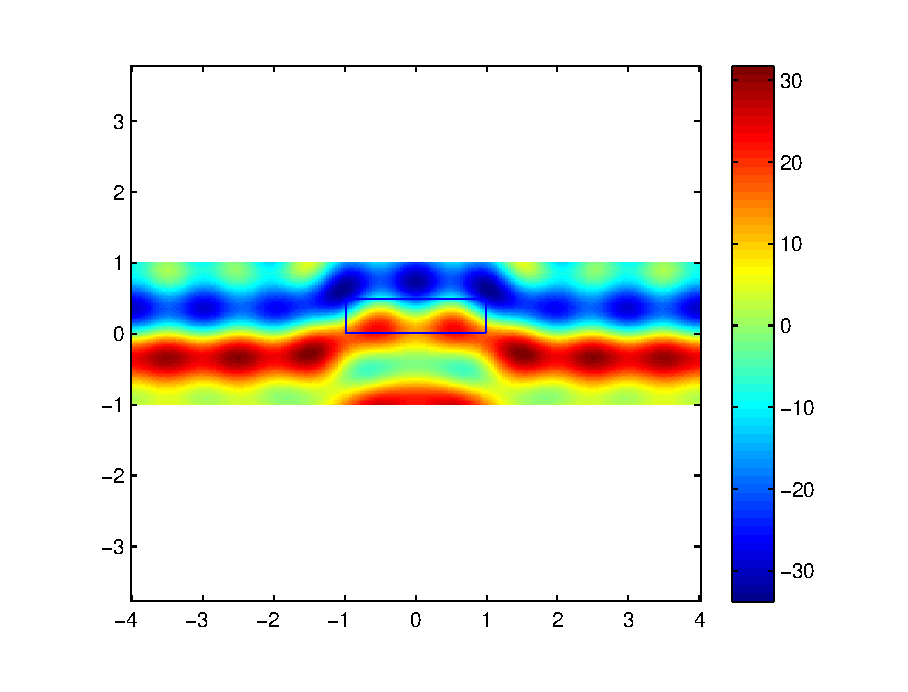
\includegraphics[width=0.8\textwidth]{./figure_rough/square_1}
	\caption{square}\label{I1}
\end{figure}
\begin{figure}
	\centering
	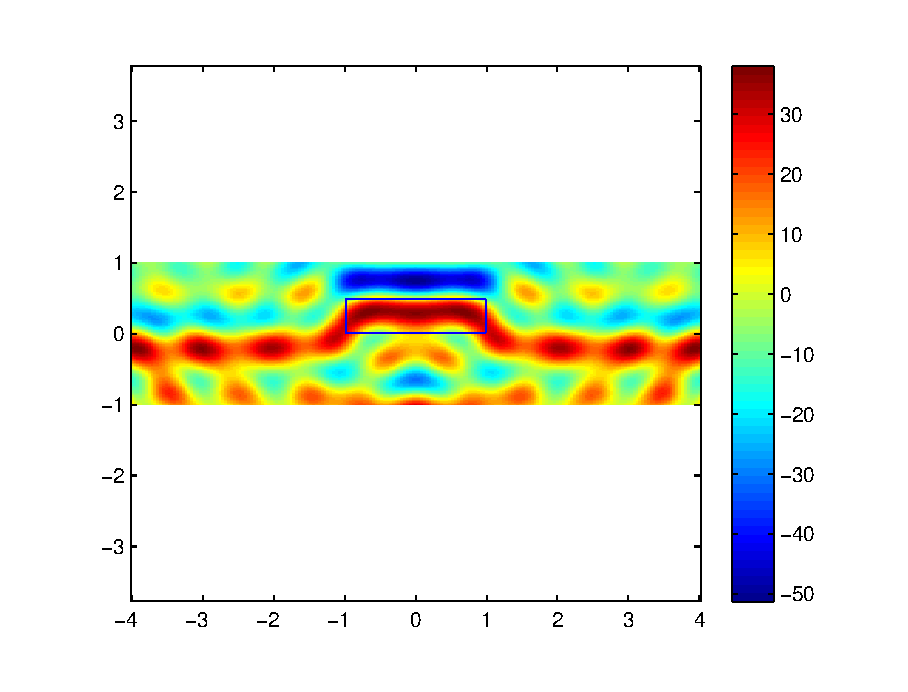
\includegraphics[width=0.8\textwidth]{./figure_rough/square_1point5}
	\caption{square}\label{I1}
\end{figure}
\begin{figure}
	\centering
	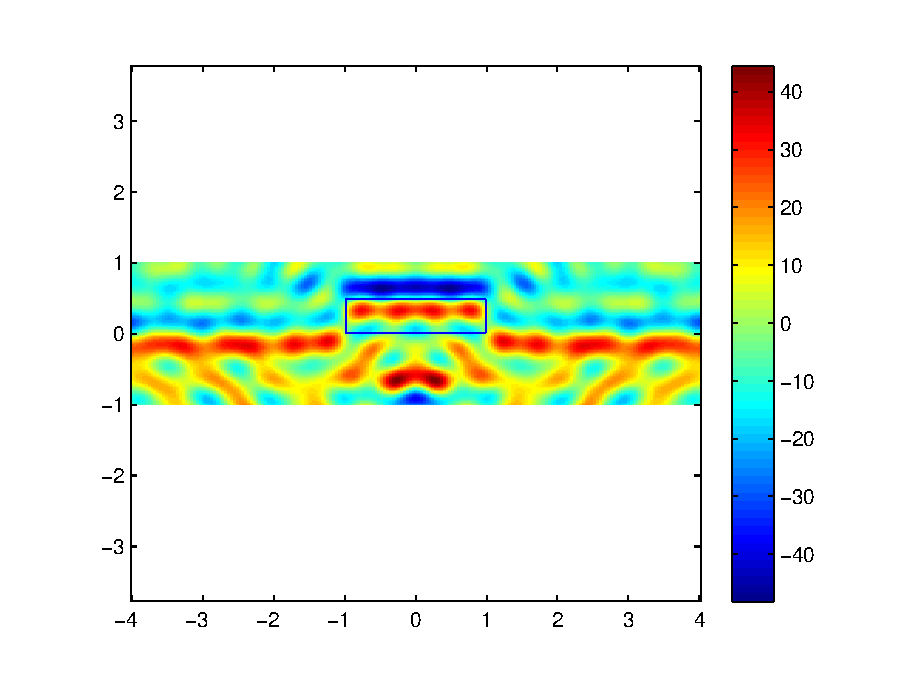
\includegraphics[width=0.8\textwidth]{./figure_rough/square_2}
	\caption{square}\label{I1}
\end{figure}
\begin{figure}
	\centering
	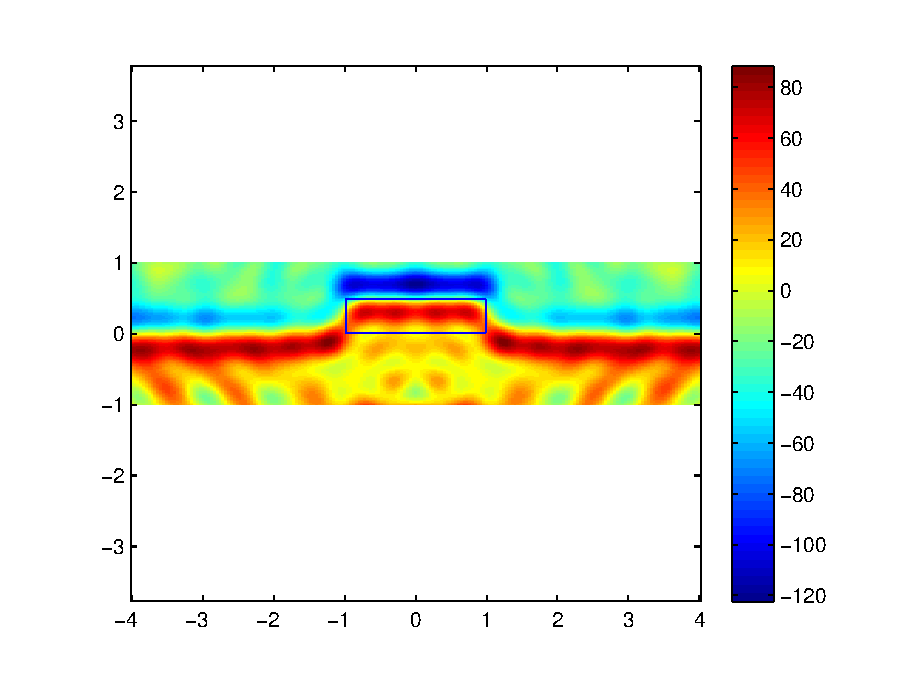
\includegraphics[width=0.8\textwidth]{./figure_rough/square_multi}
	\caption{square}\label{I1}
\end{figure}
\begin{figure}
	\centering
	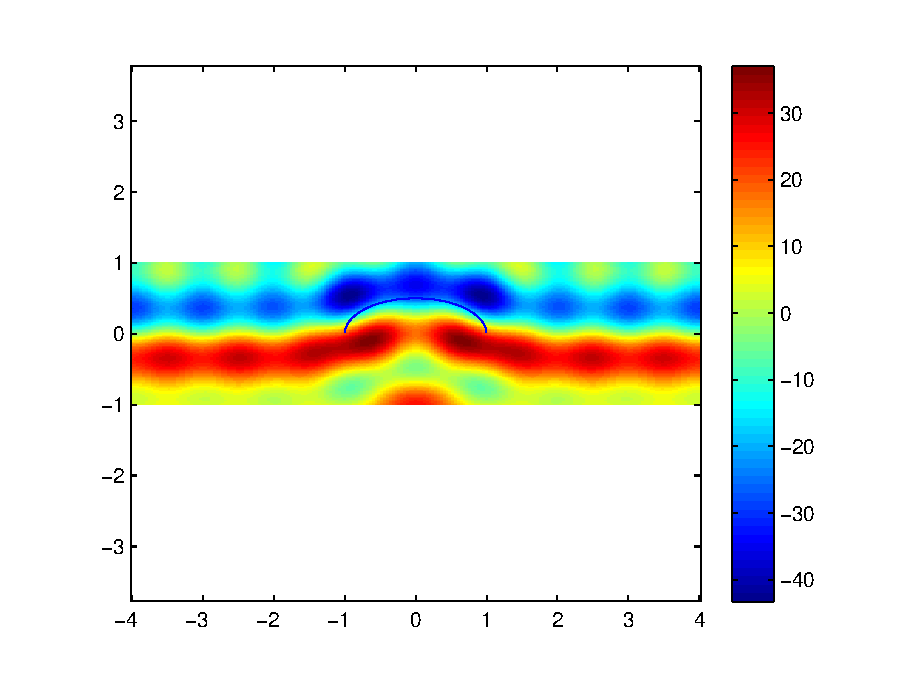
\includegraphics[width=0.8\textwidth]{./figure_rough/hemicircle_1}
	\caption{square}\label{I1}
\end{figure}
\begin{figure}
	\centering
	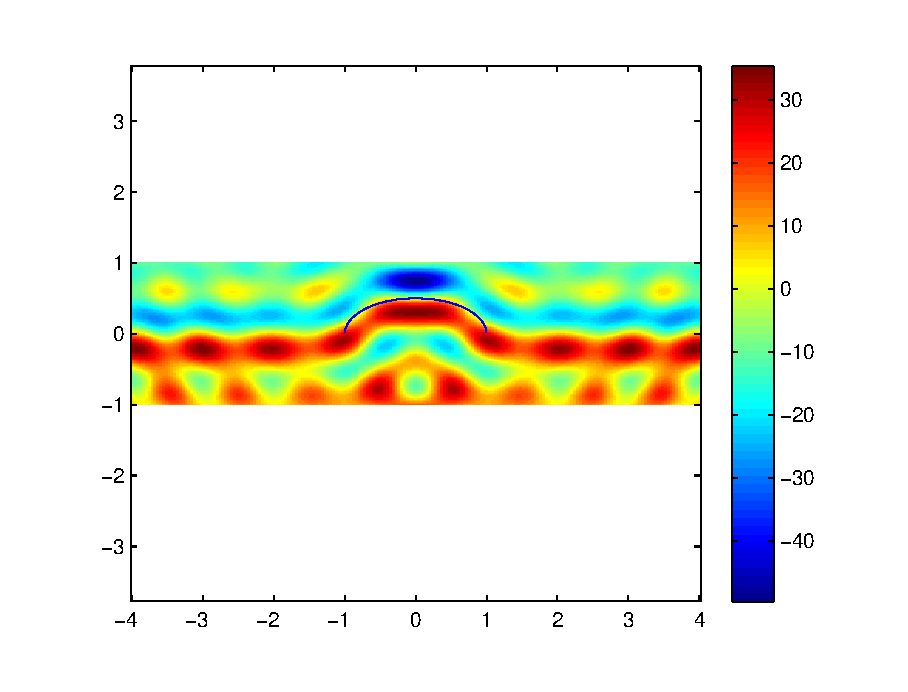
\includegraphics[width=0.8\textwidth]{./figure_rough/hemicircle_1point5}
	\caption{square}\label{I1}
\end{figure}
\begin{figure}
	\centering
	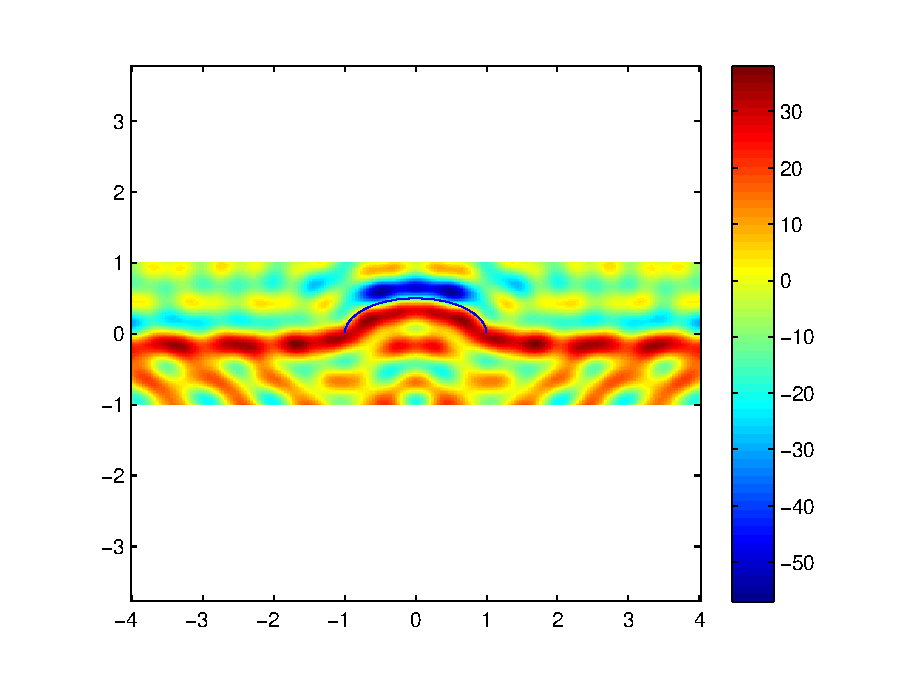
\includegraphics[width=0.8\textwidth]{./figure_rough/hemicircle_2}
	\caption{square}\label{I1}
\end{figure}
\begin{figure}
	\centering
	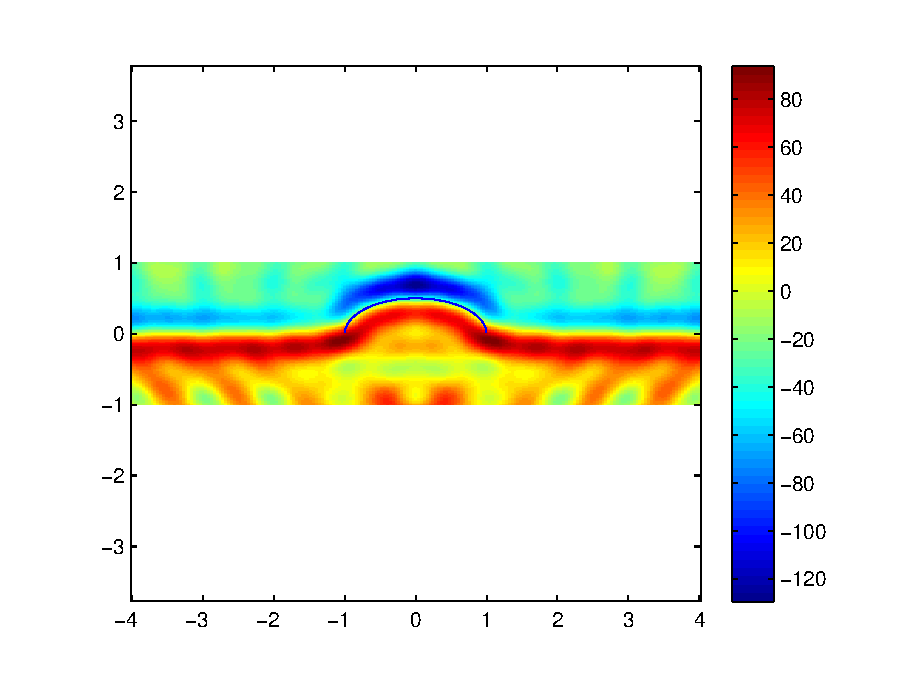
\includegraphics[width=0.8\textwidth]{./figure_rough/hemicircle_multi}
	\caption{square}\label{I1}
\end{figure}
\begin{figure}
	\centering
	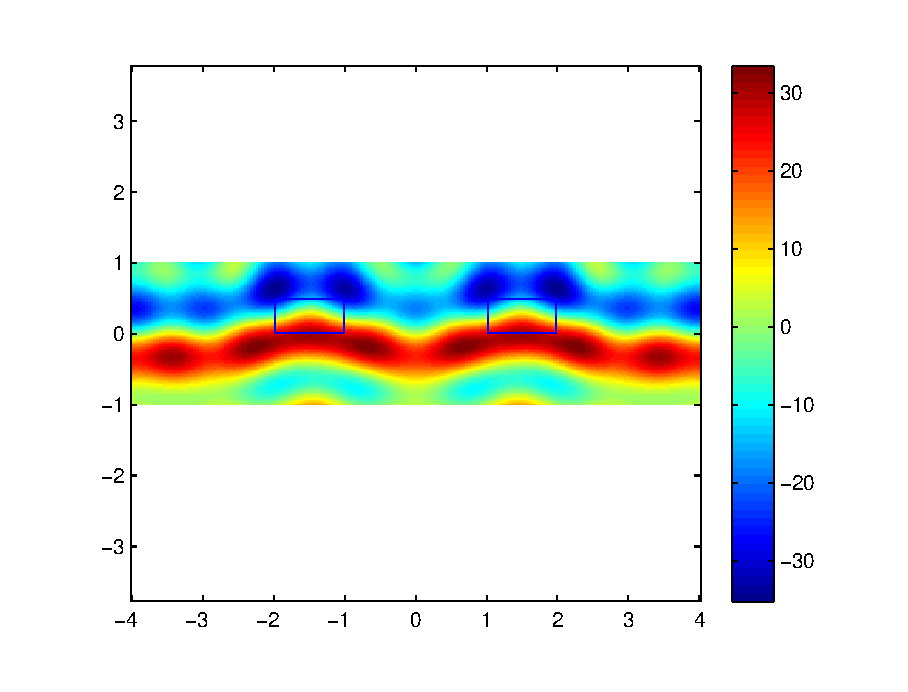
\includegraphics[width=0.8\textwidth]{./figure_rough/Bisq_1}
	\caption{square}\label{I1}
\end{figure}
\begin{figure}
	\centering
	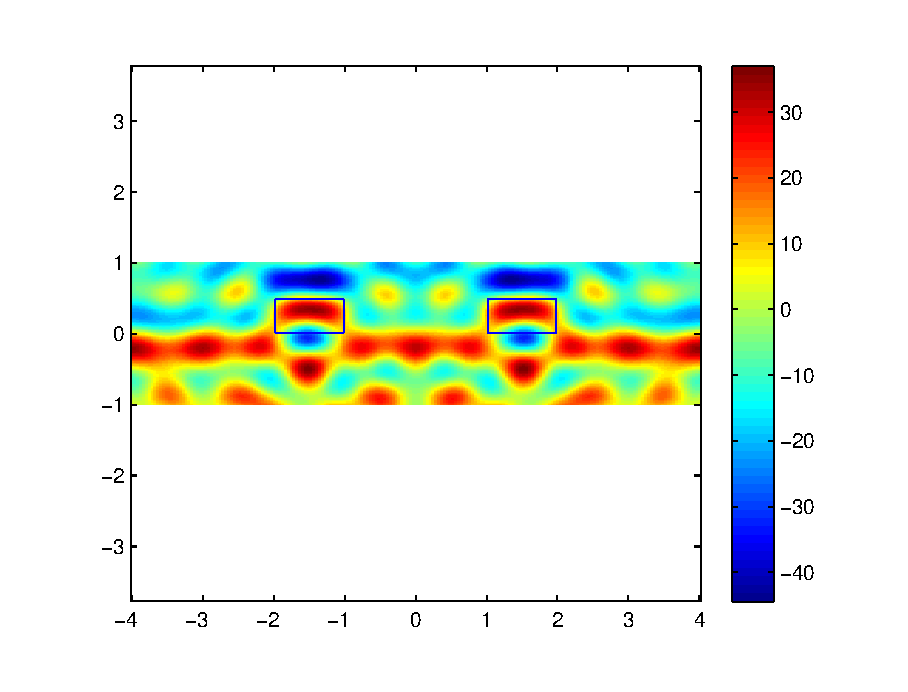
\includegraphics[width=0.8\textwidth]{./figure_rough/Bisq_1point5}
	\caption{square}\label{I1}
\end{figure}
\begin{figure}
	\centering
	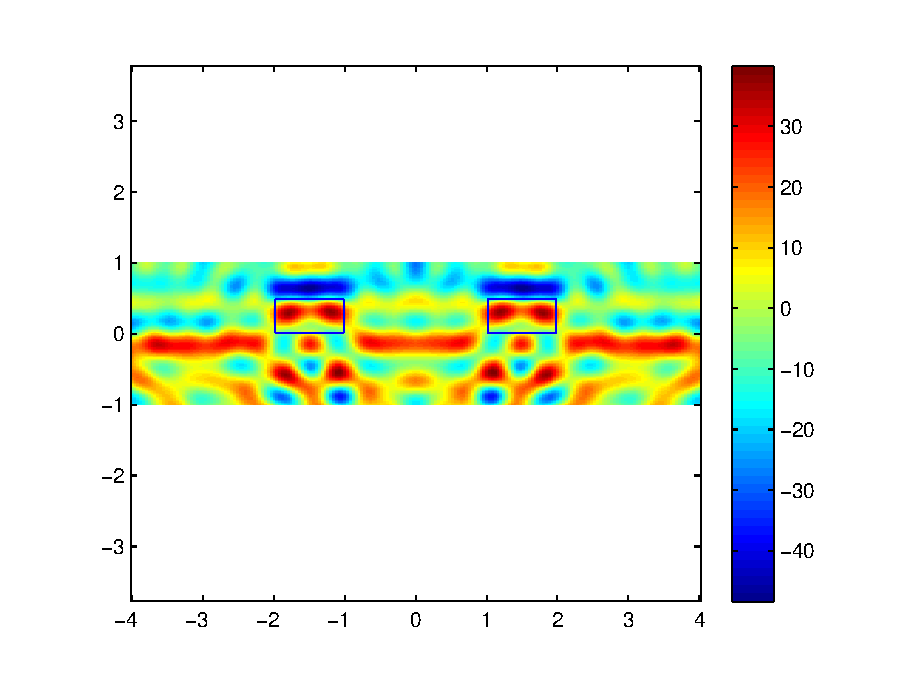
\includegraphics[width=0.8\textwidth]{./figure_rough/Bisq_2}
	\caption{square}\label{I1}
\end{figure}
\begin{figure}
	\centering
	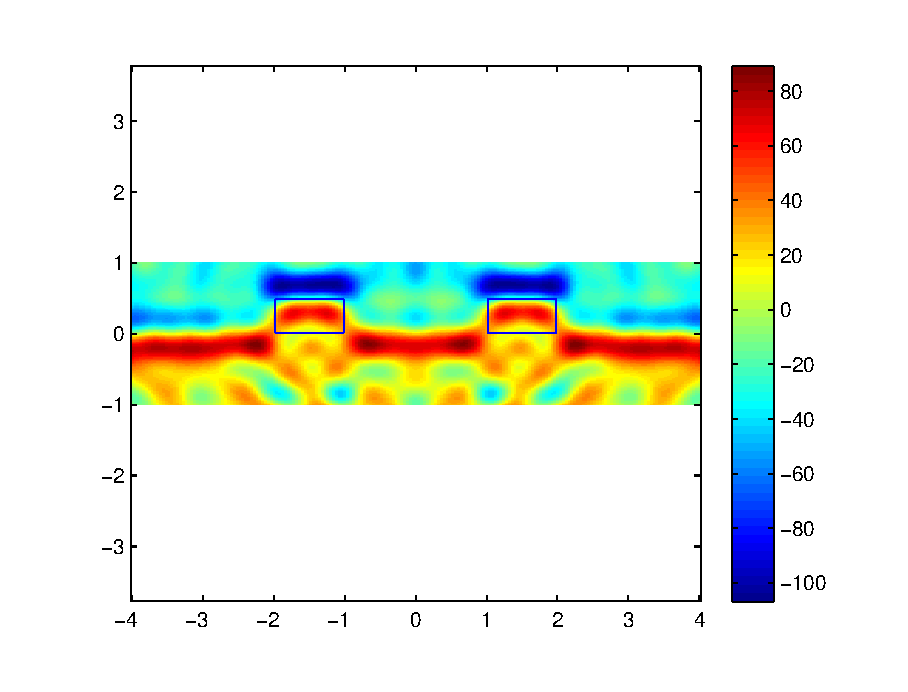
\includegraphics[width=0.8\textwidth]{./figure_rough/Bisq_multi}
	\caption{square}\label{I1}
\end{figure}
\end{document}
